\chapter{Chapter II}
\section{Teori}
\begin{enumerate}
\item \textbf{Jenis-Jenis Variabel}.\\
Variabel adalah lokasi di memori yang digunakan untuk menyimpan nilai. Pada saat kita membuat sebuah variabel, kita ‘memesan’ tempat di dalam memori. Tempat tersebut bisa diisi dengan data atau objek, baik itu bilangan bulat (integer), pecahan (float), karakter (string), dan lain – lain. Contoh:\\
	\begin{figure}[h]
	\centering
	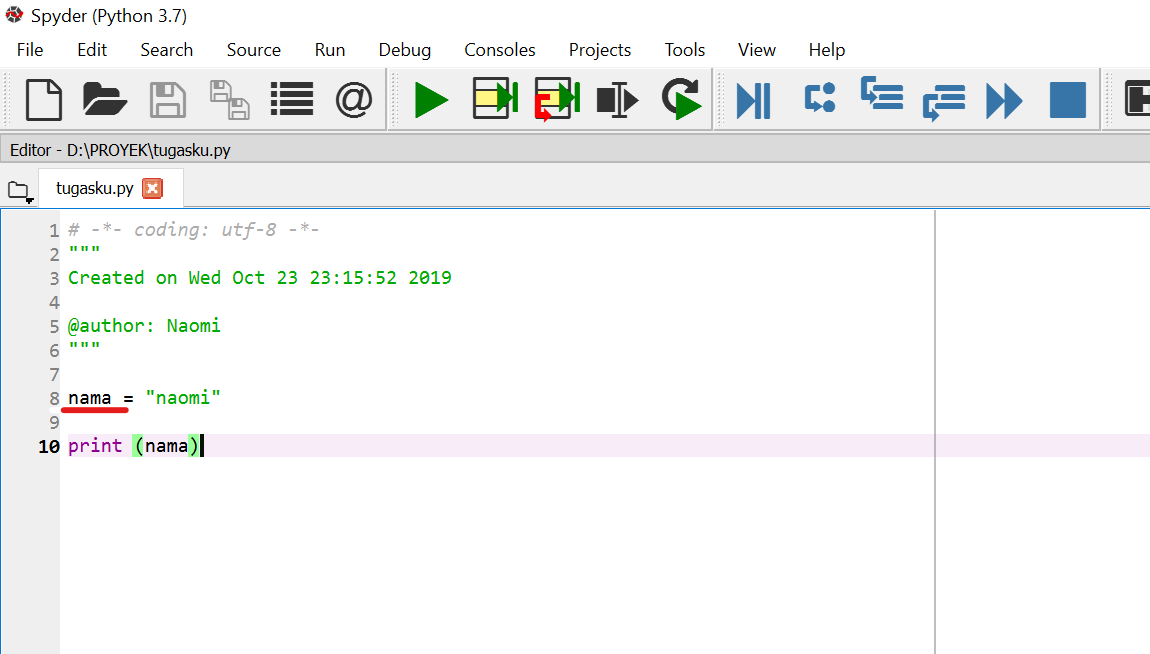
\includegraphics[width=10cm]{gambar2/cth1.png}
	\caption{contoh variabel}
	\end{figure}
	
Nama atau tanda yang diberi garis merah merupakan sebuah variabel dan "naomi" merupakan nilai dari varibel nama.\\

\item \textbf{Tipe Data}\\
    		Python memiliki enam tipe yang sering digunakan: 
\begin{itemize}
\item Bilangan (Number)
\item String
\item List
\item Set
\item Dictionary\\ Penjelasan sebagi berikut:\\

\item \textbf{Bilangan (Number)}\\
Tipe data bilangan ada dua yaitu Integer dan float. Integer ialah bilangan bulat, dan Float  bilangan pecahan. Namun masih ada jenis bilangan lain yaitu bilangan kompleks yaitu bilangan yang memiliki bagian real dan imajiner. pada python tipe data bilangan diwakili kelas int, float, complex. dan fungsi yang di pakai yaitu \textit{type()} yang digunakan untuk mengetahui tipe bilangan.\\
						\begin{figure}[!htbp]
						\centering
						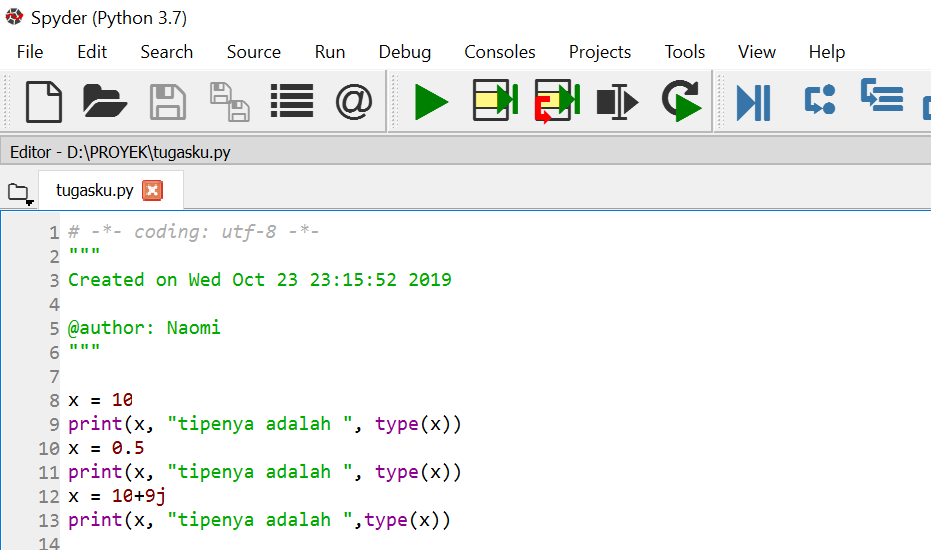
\includegraphics[width=10cm]{gambar2/cth2.png}
						\caption{contoh tipe data bilangan}
						\end{figure}\\
 Hasil:
 						\begin{figure}[!htbp]
						\centering
						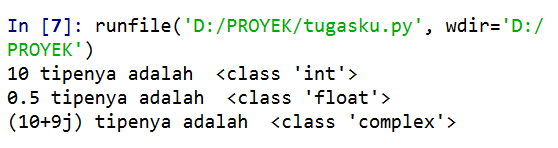
\includegraphics[width=10cm]{gambar2/hsl2.png}
						\caption{hasil contoh tipe data bilangan}
						\end{figure}\\
							
\item \textbf{String}\\
String merupakan satu atau serangkaian karakter yang diletakkan diantara tanda kutip, baik tanda kutip tunggal ( ‘ ) maupun ganda ( ” ). Huruf, angka, maupun karakter lainnya yang digabung menjadi teks adalah contoh string. String adalah tipe data yang anggotanya berurut dan memiliki indeks.\\ Indeks dimulai dari angka 0 bila dimulai dari depan dan -1 bila diindeks dari belakang. Tiap karakter bisa dilihat dari indeksnya dengan format\textit{ namastring[indeks]}. Pada tipe data ini bisa melakukan teknik slicing (memotong  nilai variabel sesuai dengan yang kita inginkan) dengan format \textit{namastring[awal:akhir]}. Contoh:
							\begin{figure}[!htbp]
							\centering
							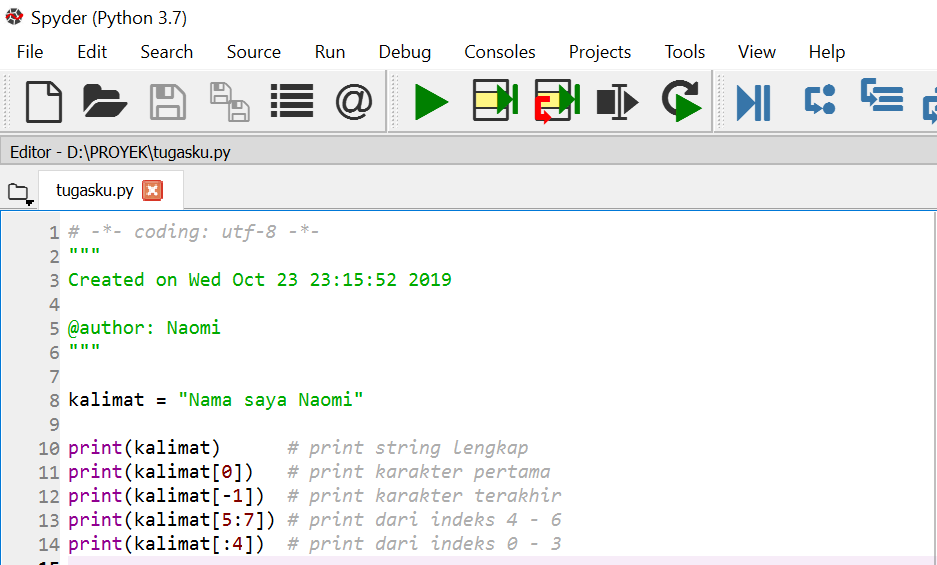
\includegraphics[width=10cm]{gambar2/cth3.png}
							\caption{contoh tipe data string}
							\end{figure}\\
Hasil:
 						\begin{figure}[!htbp]
							\centering
							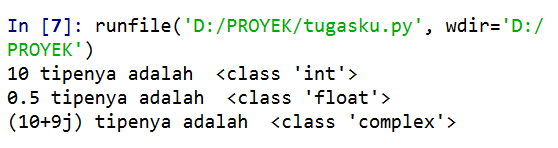
\includegraphics[width=10cm]{gambar2/hsl2.png}
							\caption{hasil contoh tipe data string}
							\end{figure}\\
							
\item \textbf{List}\\
List merupakan tipe data berisi item berurut. seperti string, tiap item (anggota) list memiliki indeks sesuai dengan urutannya masing-masing. Indeks dimulai dari awal yaitu 0 bukan 1.\\
List bisa digunakan dengan anggota tipe yang sama maupun beda. Untuk mendeklarasikan list, gunakan tanda kurung [] da masing masing anggotanya di pisahkan oleh tanda koma. \\ Untuk mengakses item dari list caranya adalah dengan memanggil nama list diikuti indeks dari item yang bersangkutan, yaitu dengan format \textit{namalist[index]} Selain itu bisa juga dilakukan pengaksesan terhadap sejumlah item dari indeks ke indeks. Contoh: \\
						\begin{figure}[!htbp]
							\centering
											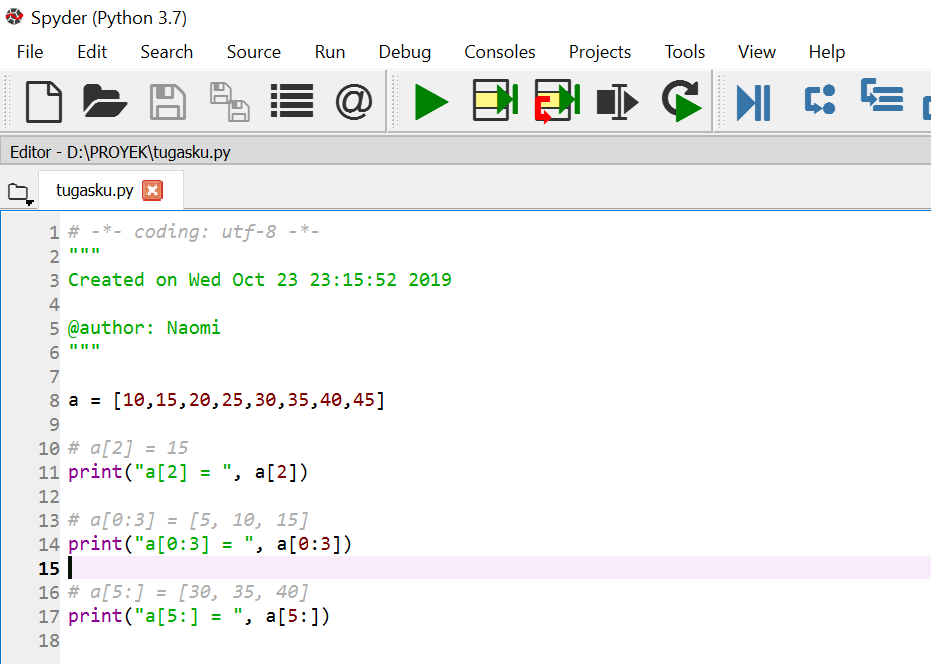
\includegraphics[width=10cm]{gambar2/cth4.png}
							\caption{contoh tipe data list}
							\end{figure}\\
Hasil:
 						\begin{figure}[!htbp]
							\centering
							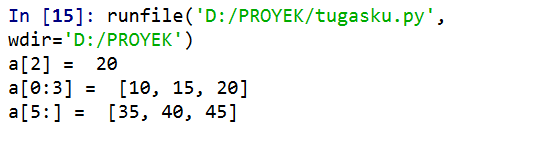
\includegraphics[width=10cm]{gambar2/hsl4.png}
							\caption{hasil contoh tipe data list}
							\end{figure}
							
\item \textbf{Set}\\
Set adalah satu tipe data di Python yang tidak berturut turut (unordered). Set memiliki anggota yang unik. Sandainya jika diletakkan dua anggota yang sama di dalam set, maka otomatis tipe data set akan menghilangkan salah satunya. Set bisa digunakan untuk melakukan operasi himpunan matematika seperti gabunga, irisan, selisih, dan komplemen.\\Set dibuat dengan meletakkan  anggota – anggotanya di dalam tanda kurung kurawal { }, dipisahkan menggunakan tanda koma. Kita juga bisa membuat set dari list dengan memasukkan list ke dalam fungsi \textit{set()}. Set bisa berisi data campuran, baik integer, float, string, dan lain sebagainya. Akan tetapi set tidak bisa berisi list, set, dan dictionary. Contoh:
\begin{figure}[!htbp]
\centering
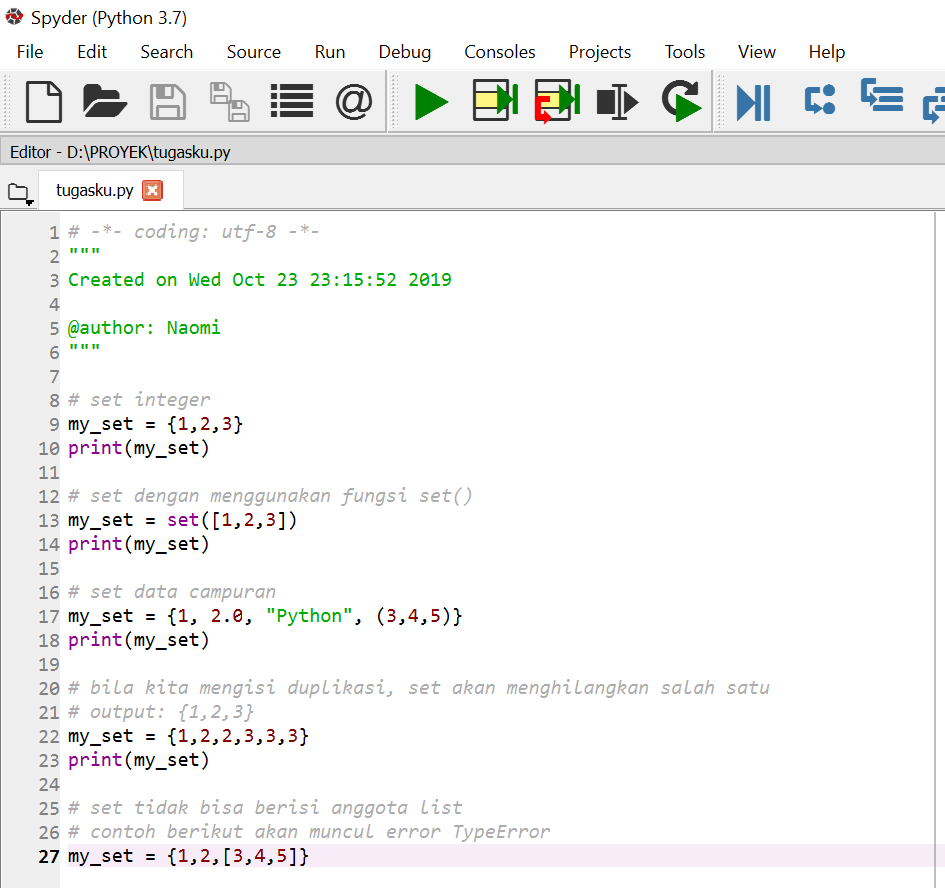
\includegraphics[width=10cm]{gambar2/cth5.png}
\caption{contoh tipe data set}
\end{figure}\\
Hasil:
\begin{figure}[!htbp]
\centering
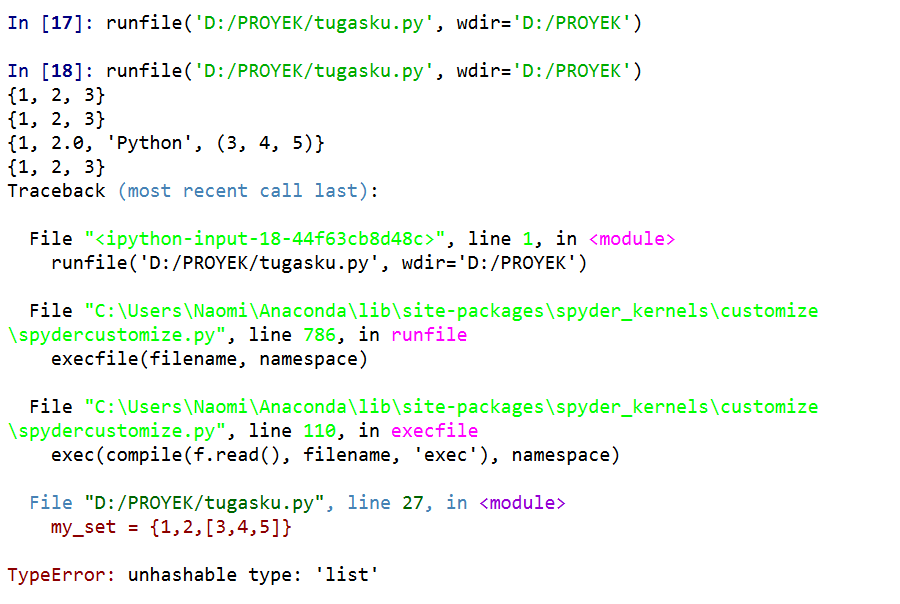
\includegraphics[width=10cm]{gambar2/hsl5.png}
\caption{hasil contoh tipe data set}
\end{figure}

\newpage
\item \textbf{Dictionary}\\
Dictionary adalah tipe data yang tiap anggotanya terdiri dari pasangan kunci-nilai (key-value). Mirip dengan kamus dimana ada kata ada arti. Dictionary umumnya dipakai untuk data yang besar dan untuk mengakses anggota data secara acak. Anggota dictionary tidak memiliki indeks. Dictionary dideklarasikan dengan menggunakan tanda kurung kurawal { }, dimana anggotanya memiliki bentuk \textit{kunci:nilai} atau \textit{key:value} dan tiap anggota dipisah tanda koma. Kunci dan nilainya bisa memiliki tipe sembarang.\\Untuk mengakses nilai dari anggota dictionary, kita menggunakan key-nya. Contoh:
\begin{figure}[!htbp]
\centering
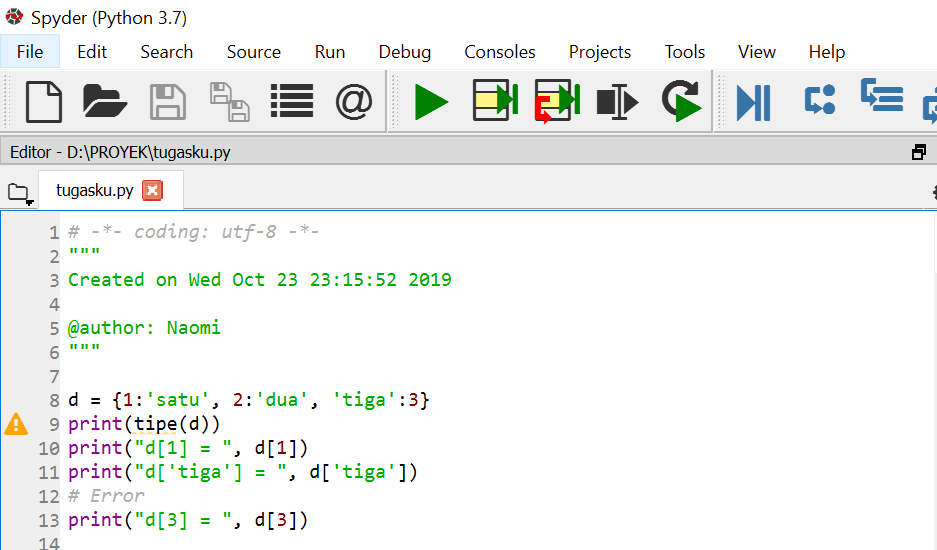
\includegraphics[width=10cm]{gambar2/cth6.png}
\caption{contoh tipe data dictionary}
\end{figure}
Hasil:
\begin{figure}[!htbp]
\centering
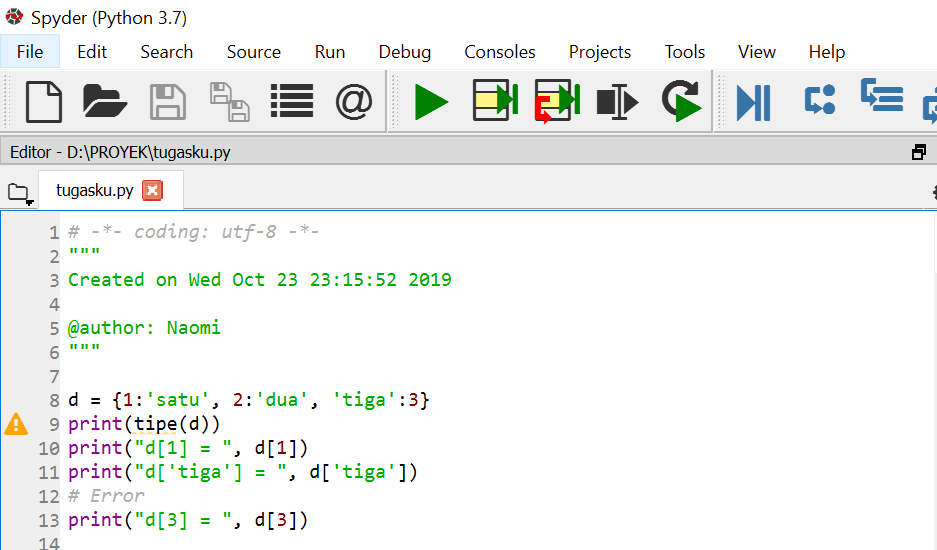
\includegraphics[width=10cm]{gambar2/cth6.png}
\caption{hasil contoh tipe data dictionary}
\end{figure}\\
\item Catatan:
\begin{itemize}
\item Tipe data sering disebut \textit{objek}. Pada dasarnya semua hal di python adalah objek.
\item Ada tipe data lain yang umumnya dimiliki oleh bahasa Python, yaitu tipe \textit{None}. Tipe \textit{None} adalah sebuah tipe data spesial yang menunjukkan bahwa nilai/data suatu variabel itu belum/tidak ada (bukan nol, tapi tidak ada). Pada bahasa pemrograman lain seperti C, atau PHP, tipe data ini disebut null.
\item Tipe data string, tuple, dan list masuk ke dalam tipe data yang disebut tipe data \textit{berurut / ordered} atau \textit{sekuensial / sequence}. Tipe data dictionary disebut data \textit{tidak berurut / unordered}.\\
\end{itemize}
\end{itemize}


\item \textbf{Input dan Output}\\
Python menyediakan banyak fungsi yang digunakan. Salah satunya adalah fungsi\textit{ i/o} atau \textit{input output}.\\
Fungsi untuk melakukan operasi output adalah \textit{print()}, dan fungsi untuk melakukan operasi input adalah fungsi \textit{input()}. 
\begin{itemize}

\item Input
\end{itemize}
Python memiliki fungsi \textit{input()}.Agar lebih memahami fungsi \textit{input()} lihat contoh berikut:
\begin{figure}[!htbp]
\centering
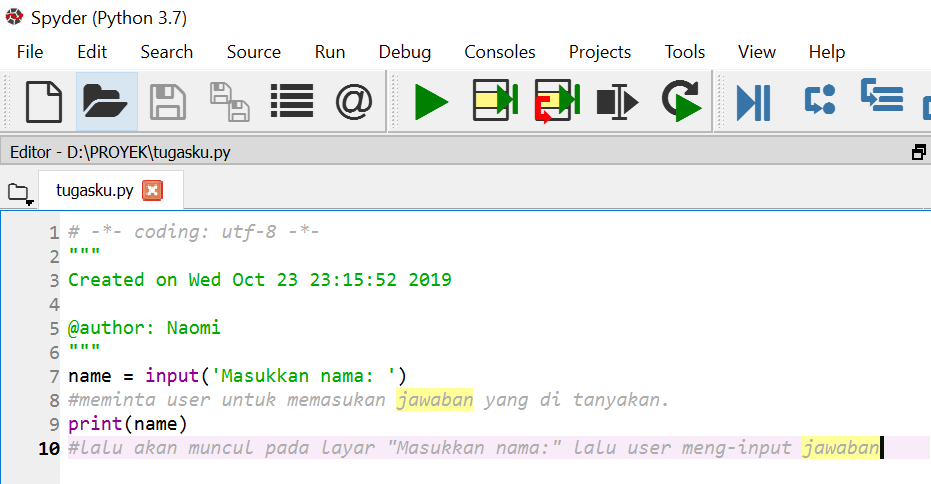
\includegraphics[width=10cm]{gambar2/cth7-1.png}
\caption{contoh fungsi input}
\end{figure}\\
    lalu akan muncul gambar seperti berikut:
\begin{figure}[!htbp]
\centering
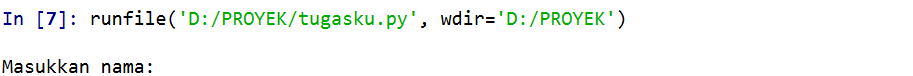
\includegraphics[width=10cm]{gambar2/cth7-2.png}
\caption{contoh fungsi input}
\end{figure}
\newpage
Hasil:
\begin{figure}[!htbp]
\centering
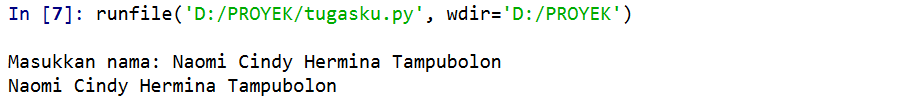
\includegraphics[width=10cm]{gambar2/hsl7.png}
\caption{hasil contoh tipe data dictionary}
\end{figure}

\begin{itemize}
\item Output
Output menggunakan fungsi \textit{print()}. Seperti yang sudah kita praktekkan, kita menggunakan fungsi\textit{ print()} untuk menampilkan data ke perangkat keluaran standar (layar). Contoh:
\begin{figure}[!htbp]
\centering
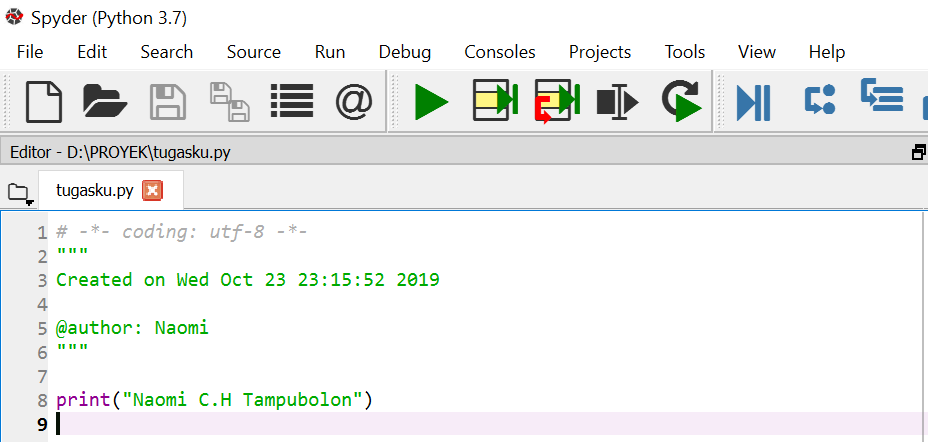
\includegraphics[width=10cm]{gambar2/cth8.png}
\caption{contoh fungsi output}
\end{figure}\\ 
Hasil:
\begin{figure}[!htbp]
\centering
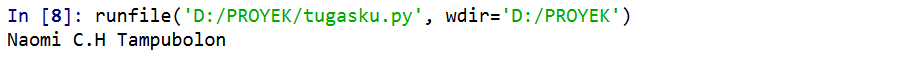
\includegraphics[width=10cm]{gambar2/hsl8.png}
\caption{hasil contoh output}
\end{figure}
\end{itemize}

\newpage
\item \textbf{Operasi dasar Aritmatika}\\
Contoh:
\begin{figure}[!htbp]
\centering
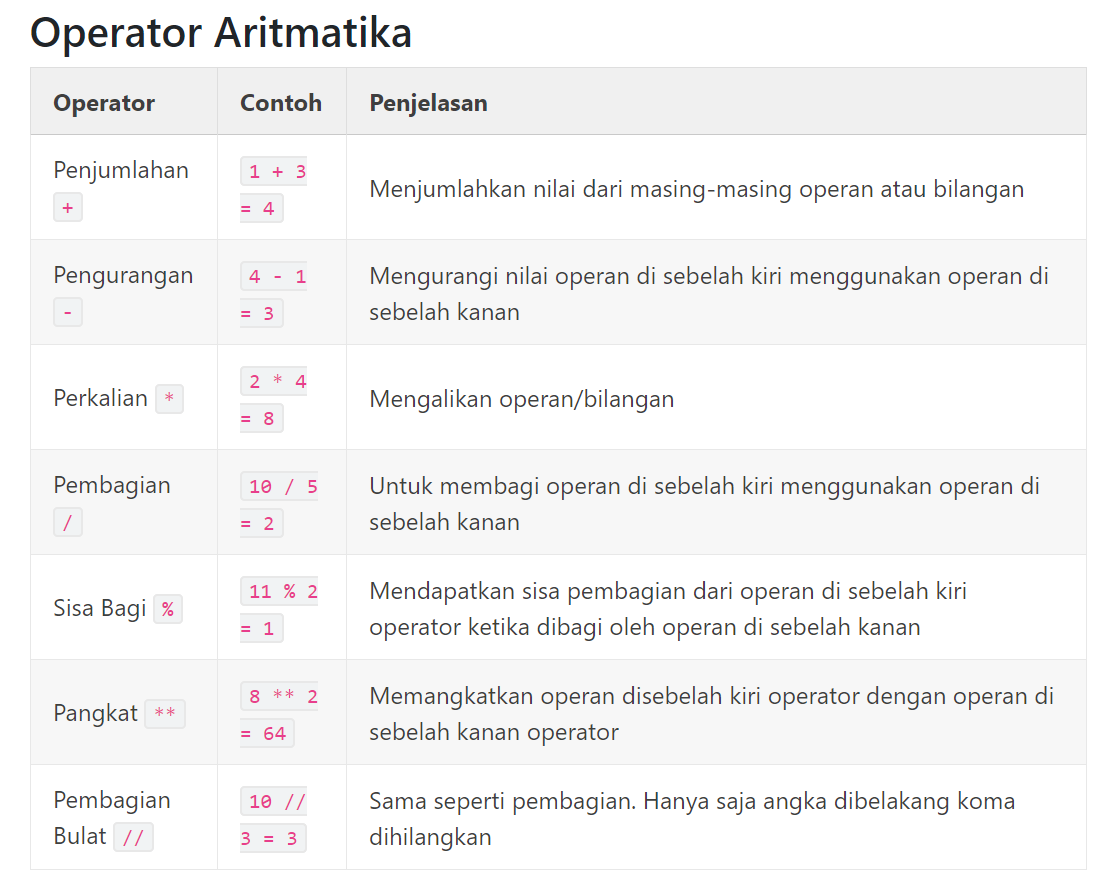
\includegraphics[width=15cm]{gambar2/cth.png}
\caption{contoh Operasi dasar Aritmatika}
\end{figure}
\begin{itemize}

\newpage
\item Penjumlahan
\begin{figure}[!htbp]
\centering
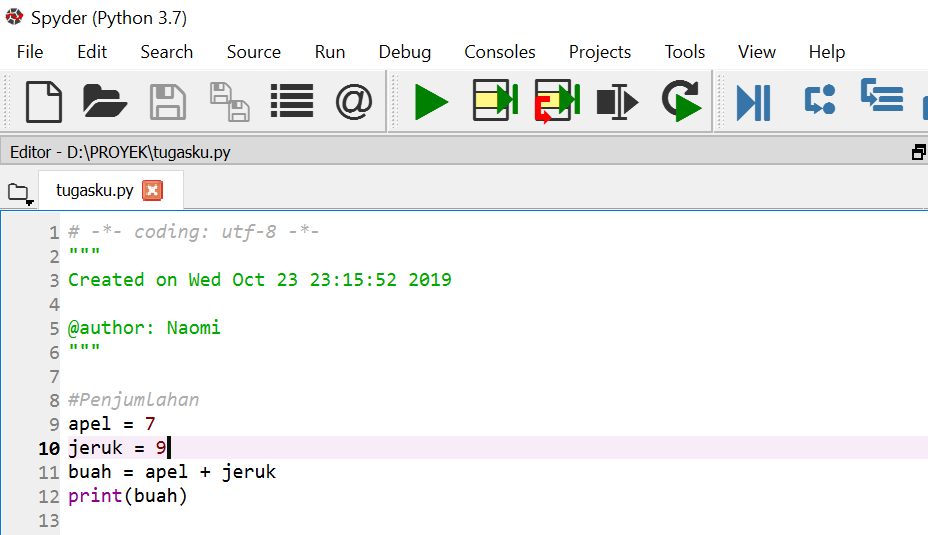
\includegraphics[width=10cm]{gambar2/tambah.png}
\caption{contoh operasi dasar aritmatika penjumlahan}
\end{figure}\\
Hasil:
\begin{figure}[!htbp]
\centering
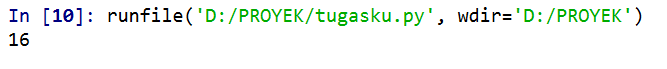
\includegraphics[width=10cm]{gambar2/tmbh1.png}
\caption{hasil contoh operasi dasar aritmatika penjumlahan}
\end{figure}

\item Pengurangan
\begin{figure}[!htbp]
\centering
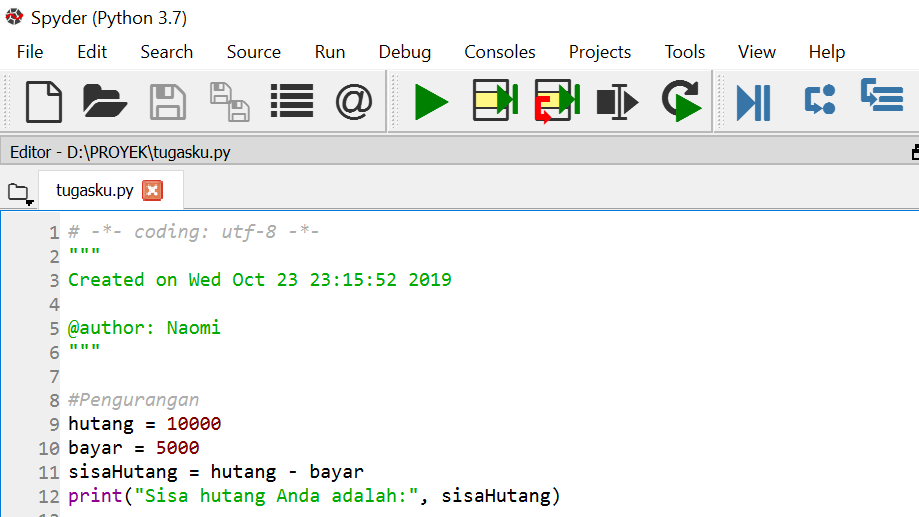
\includegraphics[width=10cm]{gambar2/kurang.png}
\caption{contoh operasi dasar aritmatika pengurangan}
\end{figure}\\
\newpage
Hasil:
\begin{figure}[!htbp]
\centering
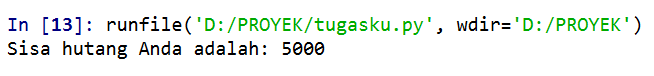
\includegraphics[width=10cm]{gambar2/krg1.png}
\caption{hasil contoh operasi dasar aritmatika pengurangan}
\end{figure}
\item Perkalian
\begin{figure}[!htbp]
\centering
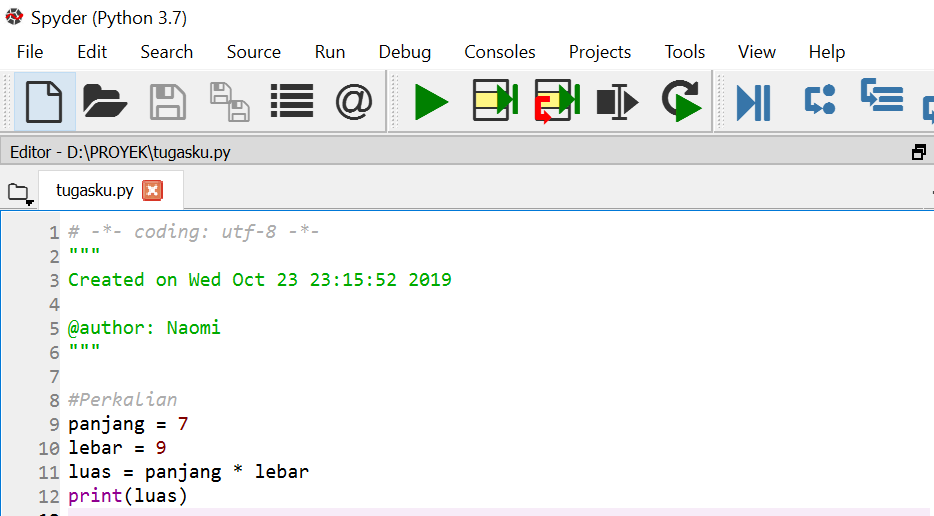
\includegraphics[width=10cm]{gambar2/kali.png}
\caption{contoh operasi dasar aritmatika perkalian}
\end{figure}\\
Hasil:
\begin{figure}[!htbp]
\centering
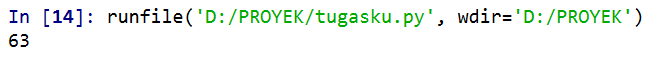
\includegraphics[width=10cm]{gambar2/kali1.png}
\caption{hasil contoh operasi dasar aritmatika perkalian}
\end{figure}

\item Pembagian
\begin{figure}[!htbp]
\centering
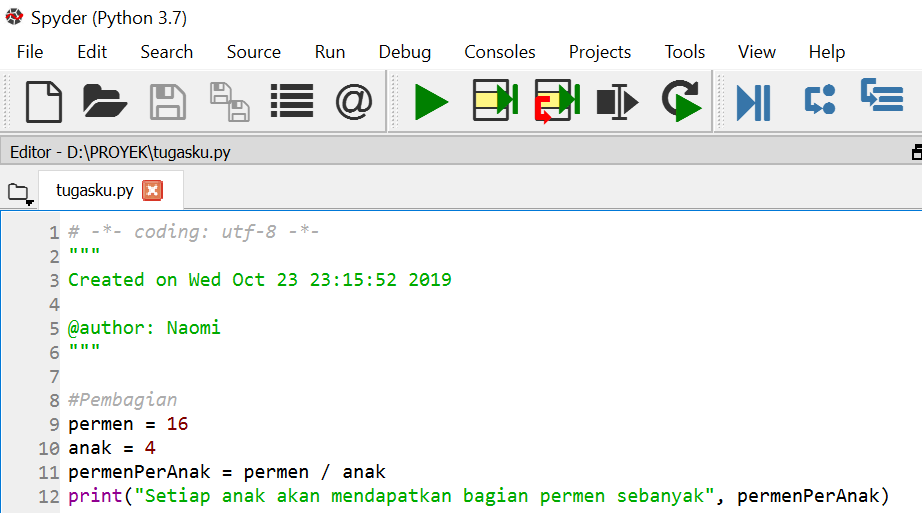
\includegraphics[width=10cm]{gambar2/bagi.png}
\caption{contoh operasi dasar aritmatika pembagian}
\end{figure}\\
\newpage
Hasil:
\begin{figure}[!htbp]
\centering
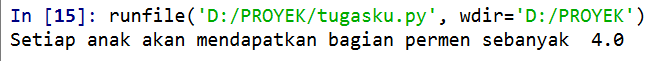
\includegraphics[width=10cm]{gambar2/bagi1.png}
\caption{hasil contoh operasi dasar aritmatika pembagian}
\end{figure}

\item Sisa Bagi
\begin{figure}[!htbp]
\centering
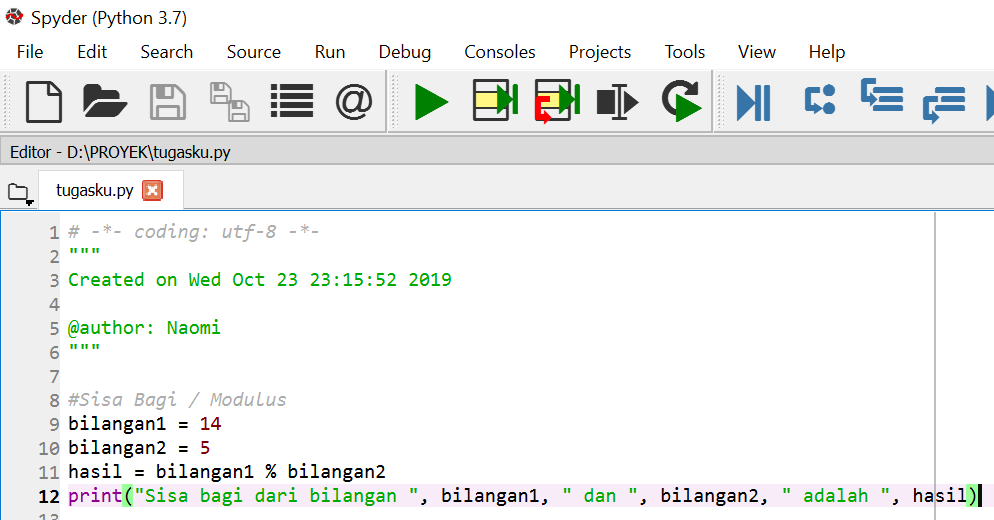
\includegraphics[width=10cm]{gambar2/modulus.png}
\caption{contoh operasi dasar aritmatika sisa bagi}
\end{figure}\\
Hasil:
\begin{figure}[!htbp]
\centering
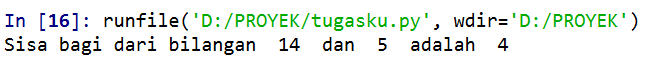
\includegraphics[width=10cm]{gambar2/modulus1.png}
\caption{hasil contoh operasi dasar aritmatika sisa bagi}
\end{figure}

\item Pangkat
\begin{figure}[!htbp]
\centering
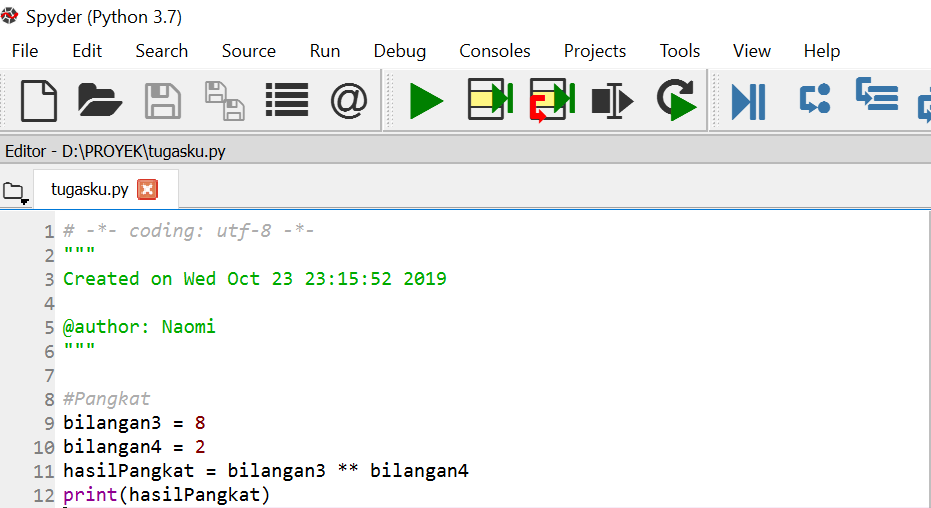
\includegraphics[width=10cm]{gambar2/pangkat.png}
\caption{contoh operasi dasar aritmatika pangkat}
\end{figure}
\newpage
Hasil:
\begin{figure}[!htbp]
\centering
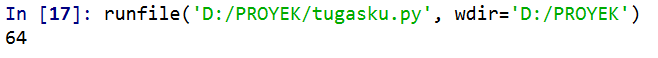
\includegraphics[width=10cm]{gambar2/pangkat1.png}
\caption{hasil contoh operasi dasar aritmatika pangkat}
\end{figure}

\item Pembagian Bulat
\begin{figure}[!htbp]
\centering
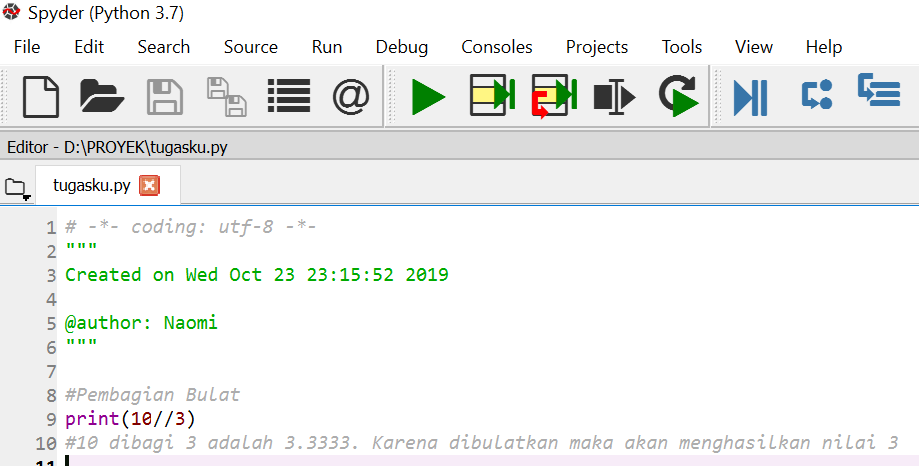
\includegraphics[width=10cm]{gambar2/bulat.png}
\caption{contoh operasi dasar aritmatika pembagian bulat}
\end{figure}\\
Hasil:
\begin{figure}[!htbp]
\centering
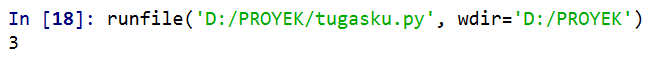
\includegraphics[width=10cm]{gambar2/bulat1.png}
\caption{hasil contoh operasi dasar aritmatika pembagian bulat}
\end{figure}
\end{itemize}

\item \textbf{Perulangan (Looping)}\\
Perulangan dalam bahasa pemrograman berfungsi menyuruh komputer melakukan sesuatu secara berulang-ulang. Terdapat dua jenis perualangan dalam bahasa pemrograman python, yaitu perulangan dengan \textit{for, while} dan \textit{nasted}.
\begin{itemize}
\item Perulangan For\\
Pengulangan \textit{for} pada Python memiliki kemampuan untuk mengulangi item dari urutan apapun, seperti \textit{list} atau \textit{string}. Contoh:
\begin{figure}[!htbp]
\centering
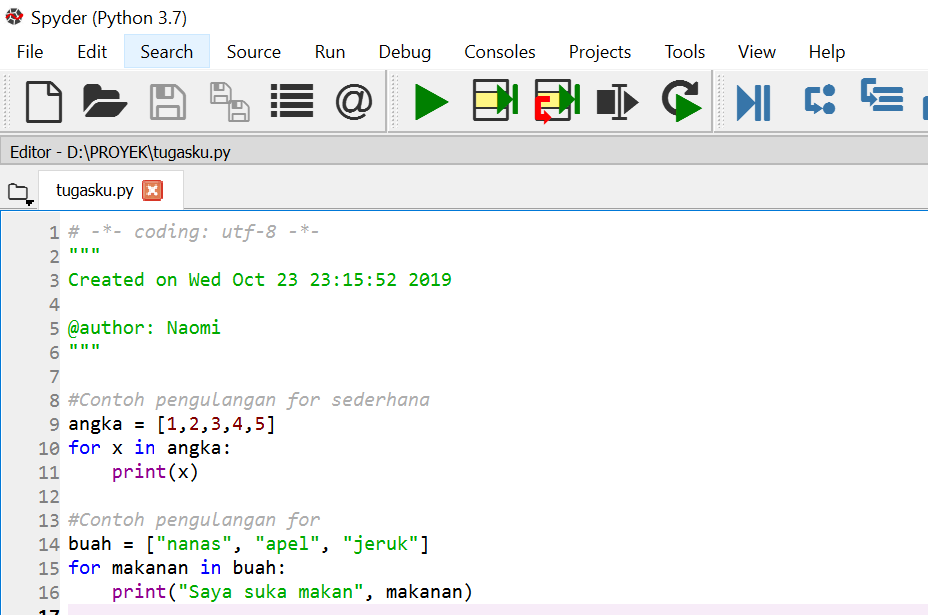
\includegraphics[width=13cm]{gambar2/for.png}
\caption{contoh perulangan for}
\end{figure}
\newpage
Hasil:
\begin{figure}[!htbp]
\centering
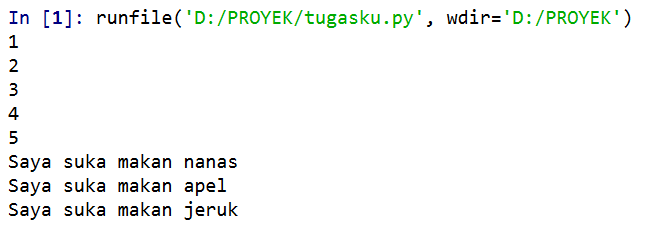
\includegraphics[width=13cm]{gambar2/for1.png}
\caption{hasil contoh perulang For}
\end{figure}
\newpage
\item Perulangan While\\
Pengulangan While di dalam bahasa pemrograman Python yaitu dieksesusi berkali-kali selama kondisi bernilai benar atau \textit{True}. Contoh:
\begin{figure}[!htbp]
\centering
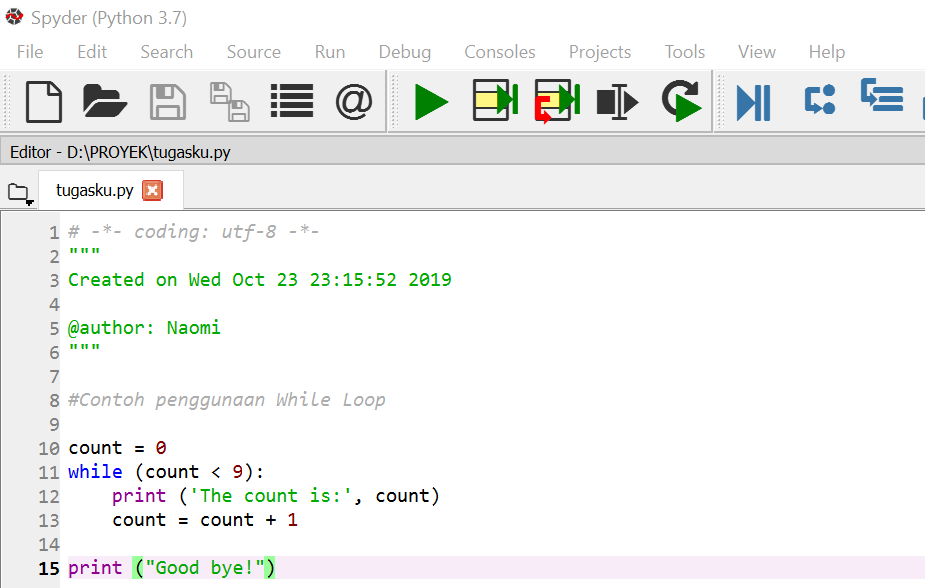
\includegraphics[width=13cm]{gambar2/while.png}
\caption{contoh perulangan while}
\end{figure}
Hasil:
\begin{figure}[!htbp]
\centering
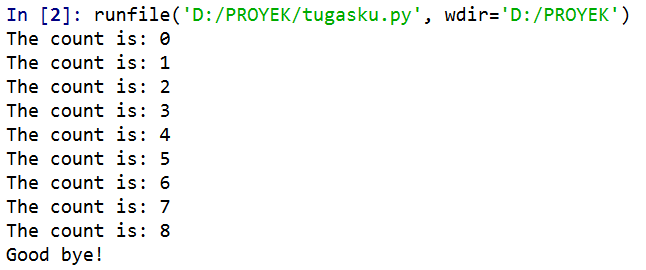
\includegraphics[width=13cm]{gambar2/while1.png}
\caption{hasil contoh perulang While}
\end{figure}
\newpage
\item Nasted\\
Nasted jarang digunakan. Contoh Nasted adalah:
\begin{figure}[!htbp]
\centering
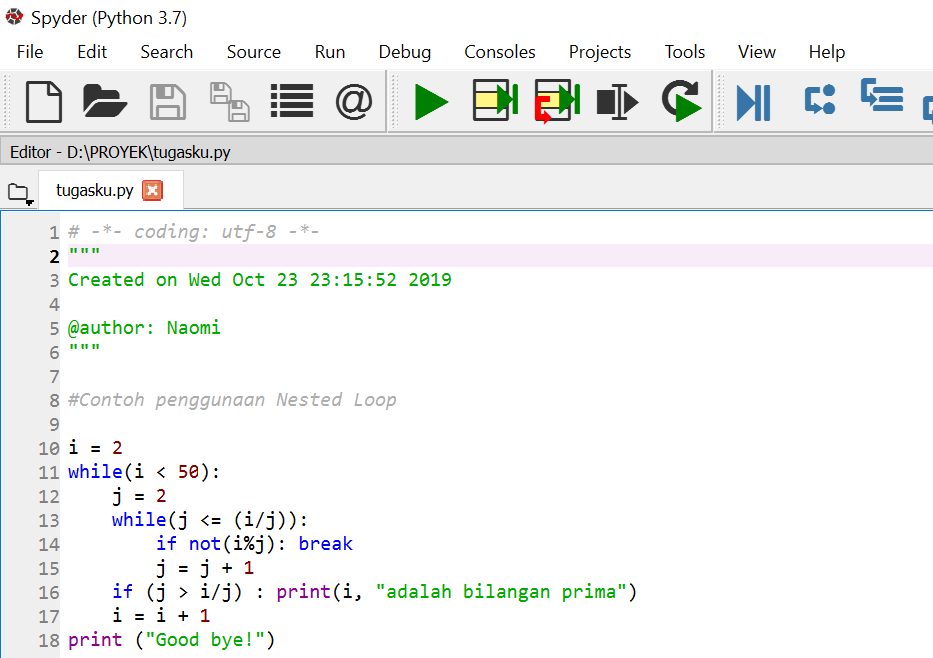
\includegraphics[width=13cm]{gambar2/nasted.png}
\caption{contoh perulangan nasted}
\end{figure}\\
Hasil:
\begin{figure}[!htbp]
\centering
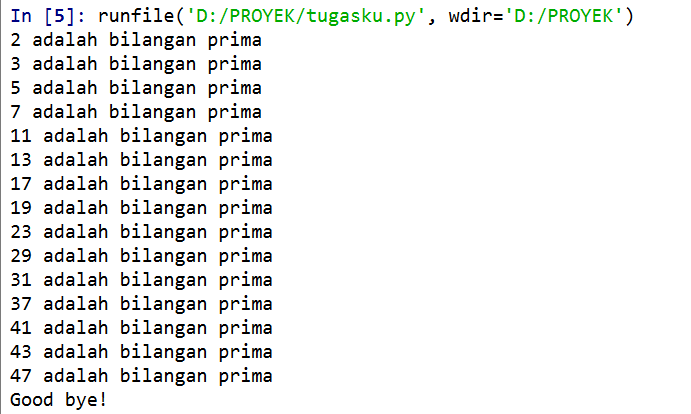
\includegraphics[width=13cm]{gambar2/nasted1.png}
\caption{hasil contoh perulang nasted}
\end{figure}
\end{itemize}

\newpage
\item \textbf{Kondisi}\\
    Kodisi ada 3(tiga) yaitu:
    \begin{figure}[!htbp]
    \centering
    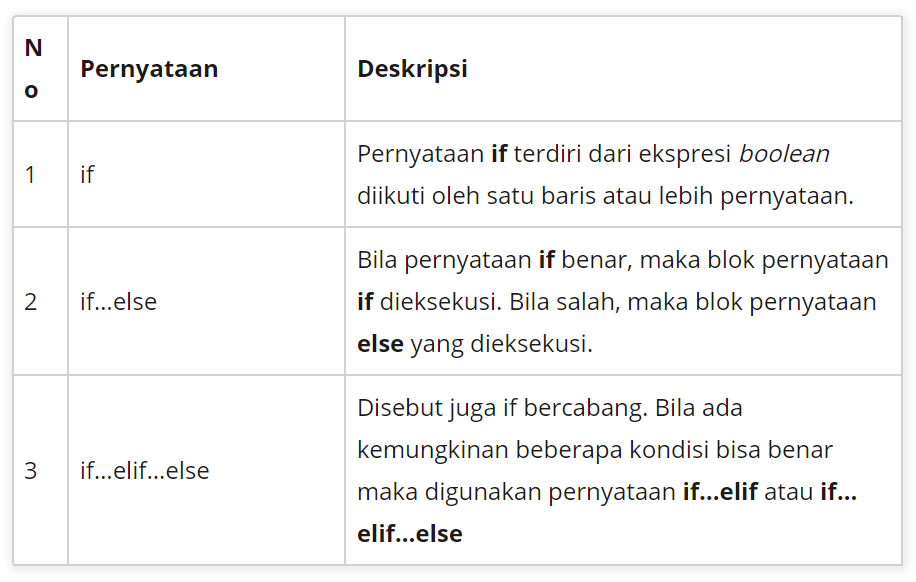
\includegraphics[width=9cm]{gambar2/cthkondisi.png}
    \caption{Kondisi IF}
    \end{figure}
    \begin{itemize}
        \item Kondisi IF\\
        Pernyataan if menguji satu buah kondisi. Bila hasilnya benar maka pernyataan di dalam blok if tersebut dieksekusi. Bila salah, maka pernyataan tidak dieksekusi. contoh:
    \begin{figure}[!htbp]
    \centering
    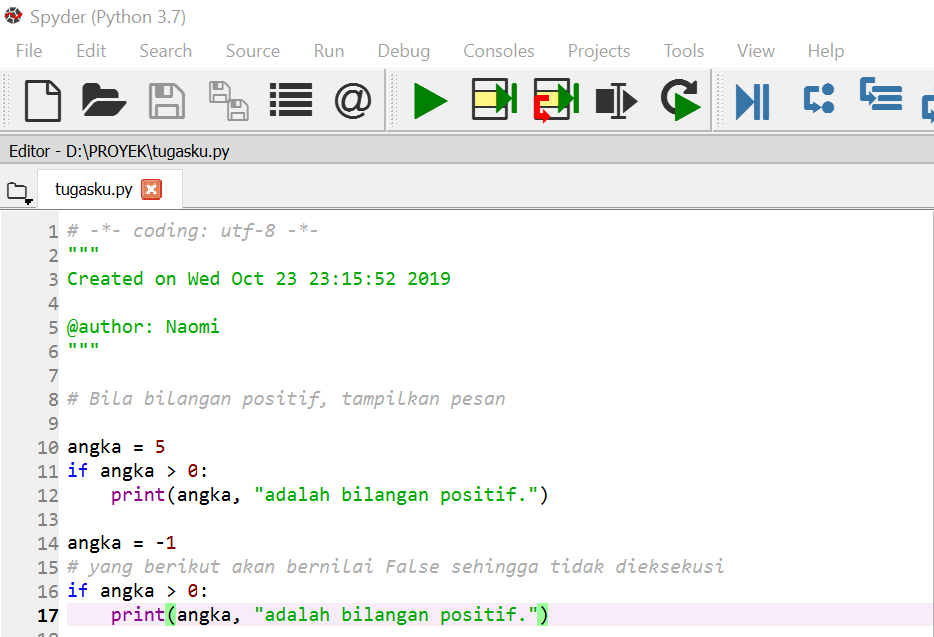
\includegraphics[width=9cm]{gambar2/if.png}
    \caption{kondisi IF}
    \end{figure}
    Hasil:
    \begin{figure}[!htbp]
    \centering
    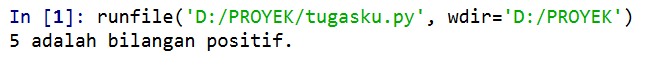
\includegraphics[width=10cm]{gambar2/if1.png}
    \caption{kondisi IF}
    \end{figure}
    \newpage
        Pada contoh di atas, awalnya angka berisi 5. Pada saat if yang pertama dieksekusi maka kondisinya adalah apakah 5 lebih besar dari 0? Karena hasilnya benar/True, maka statement di grup if ini dieksekusi dan menampilkan pesan 5 adalah bilangan positif.\\
        Selanjutnya angka sudah diubah jadi -1. Untuk if yang kedua, hasil pengujian kondisinya menjadi apakah -1 lebih besar dari 0? Hasilnya salah/False. Oleh karena itu, pernyataan di dalam grupnya tidak dijalankan.

        \item Kondisi IF ELSE\\
        Pernyataan if…else menguji 2 kondisi. Kondisi pertama kalau benar, dan kondisi kedua kalau salah. Contoh:
    \begin{figure}[!htbp]
    \centering
    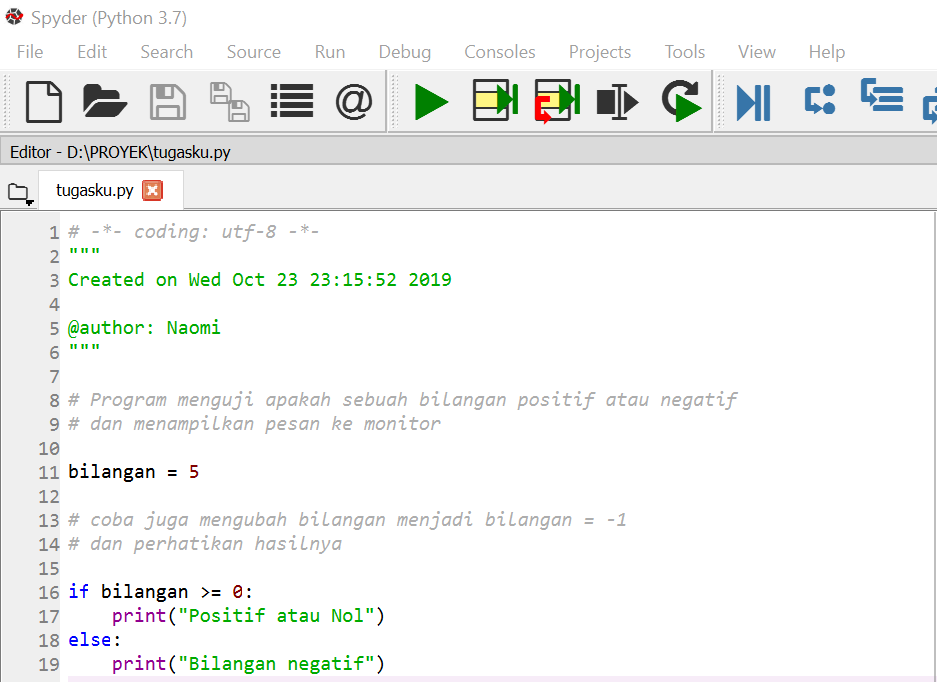
\includegraphics[width=10cm]{gambar2/ifelse.png}
    \caption{kondisi IF ELSE}
    \end{figure}\\
    Hasil:
    \begin{figure}[!htbp]
    \centering
    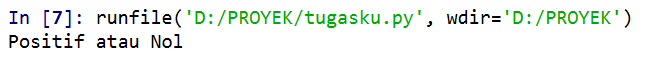
\includegraphics[width=10cm]{gambar2/ifelse1.png}
    \caption{kondisi IF ELSE}
    \end{figure}
    \newpage
        Pada contoh di atas, bilangan kita beri nilai 5. Kemudian pada pengujian if, kondisinya adalah apakah bilangan >= 0? Hasilnya adalah benar, maka hasil yang ditampilkan adalah Positif atau Nol. Seandainya kita ganti bilangan jadi -1, maka hasil pengujian if nya akan salah/False dan blok else yang akan dijalankan, yaitu menampilkan pesan Bilangan negatif
        \item Kondisi \textit{IF ELIF ELSE}\\
        Pernyataan if elif else digunakan untuk menguji lebih dari 2 kondisi. Bila kondisi pada if benar, maka pernyataan di dalamnya yang dieksekusi. Bila salah, maka masuk ke pengujian kondisi elif. Terakhir bila tidak ada if atau elif yang benar, maka yang dijalankan adalah yang di blok else. Contoh:
    \begin{figure}[!htbp]
    \centering
    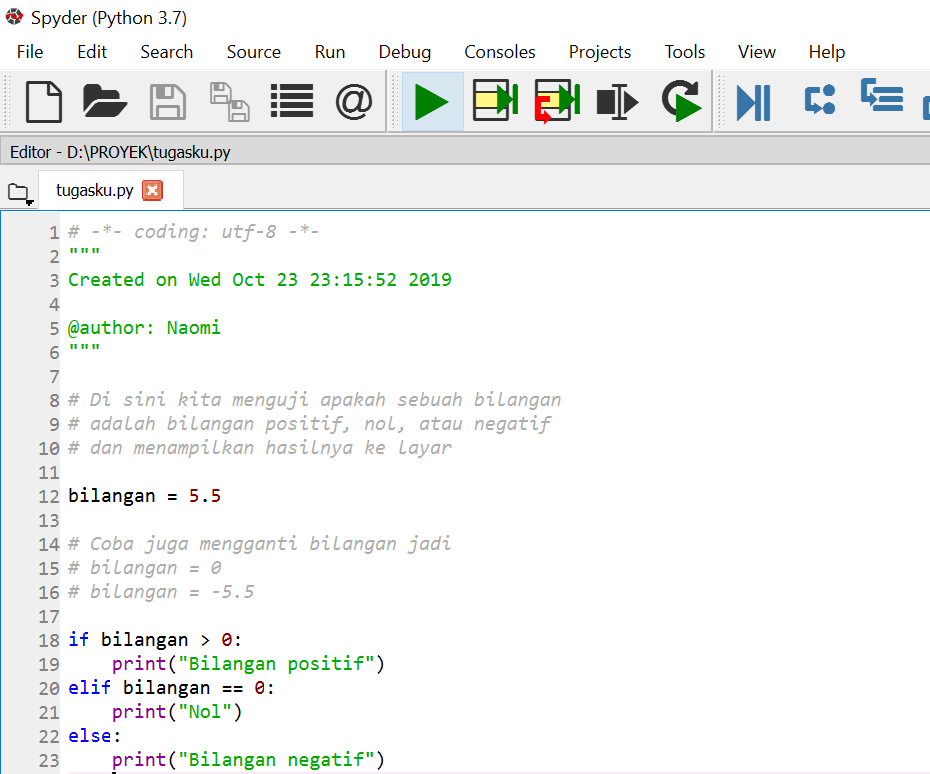
\includegraphics[width=10cm]{gambar2/ifelifelse.png}
    \caption{kondisi IF ELIF ELSE}
    \end{figure}\\
    Hasil:
    \begin{figure}[!htbp]
    \centering
    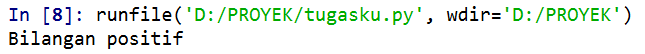
\includegraphics[width=10cm]{gambar2/ifelifelse1.png}
    \caption{kondisi IF ELIF ELSE}
    \end{figure}
    \newpage
        Pada contoh di atas, bilangan kita beri nilai 5.5. Pada pengujian if, kondisinya adalah apakah bilangan lebih besar 0? Hasilnya benar, maka yang ditampilkan adalah pesan Bilangan positif.\\
        Bila nilai bilangan kita ganti menjadi 0, maka yang akan bernilai benar adalah pernyataan elif. Bila kita menggantikan bilangan jadi minus, maka kondisi if dan elif salah, dan yang dijalankan adalah blok else.
    \item Catatan:
        Python mengasumsikan bahwa nilai selain nol dan selain tipe None sebagai nilai True, dan yang nilai nol dan None sebagai False.
    \end{itemize}

\item Sintaks Error
Contoh Sintaks yang error:
    \begin{figure}[!htbp]
    \centering
    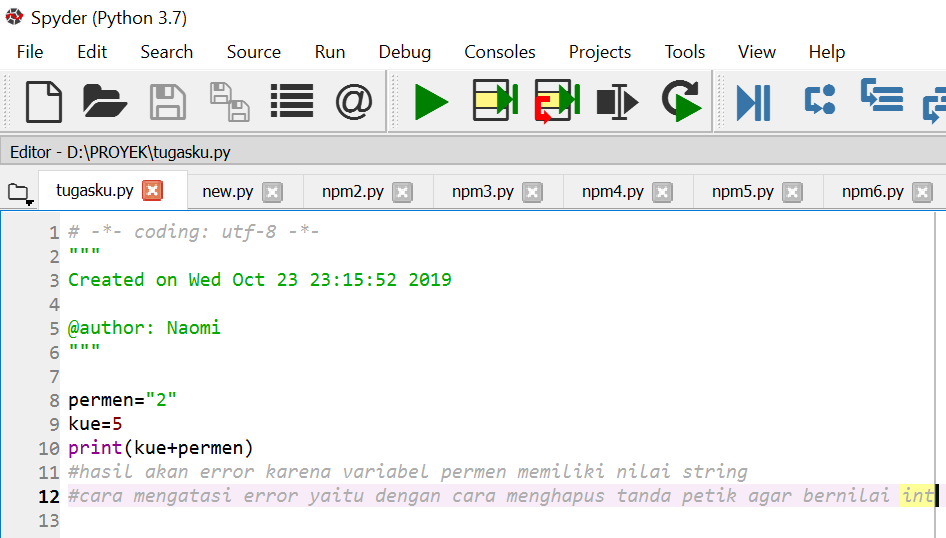
\includegraphics[width=9cm]{gambar2/error.png}
    \caption{Contoh Sintaks Error}
    \end{figure}\\
    Hasil:
    \begin{figure}[!htbp]
    \centering
    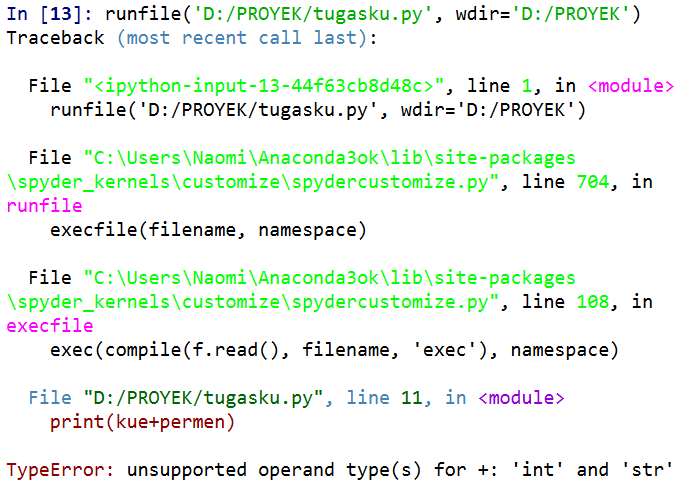
\includegraphics[width=9cm]{gambar2/error1.png}
    \caption{Hasil Contoh Sintaks Error}
    \end{figure}
\newpage
\item Try Except
    \begin{figure}[!htbp]
    \centering
    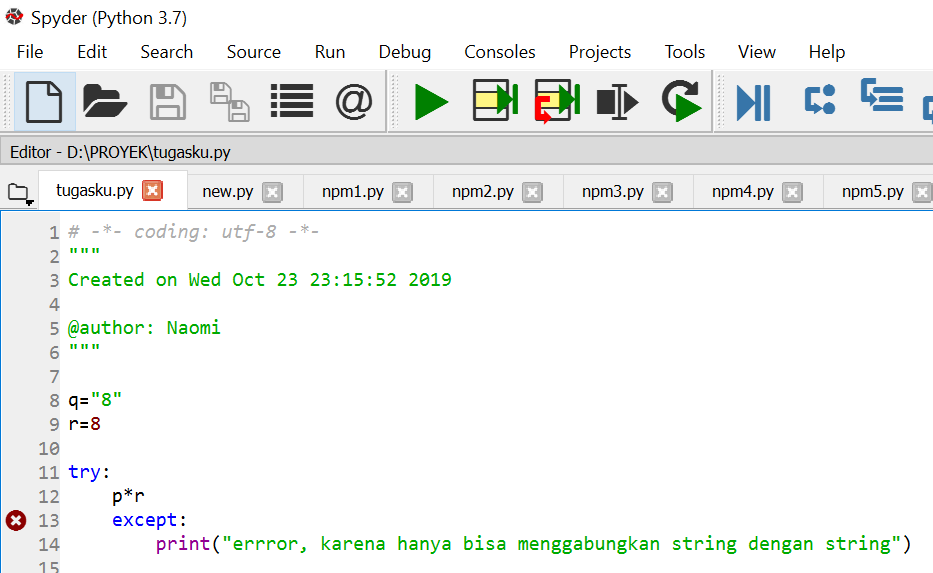
\includegraphics[width=10cm]{gambar2/try.png}
    \caption{Contoh Try Except}
    \end{figure}\\
    Hasil:
    \begin{figure}[!htbp]
    \centering
    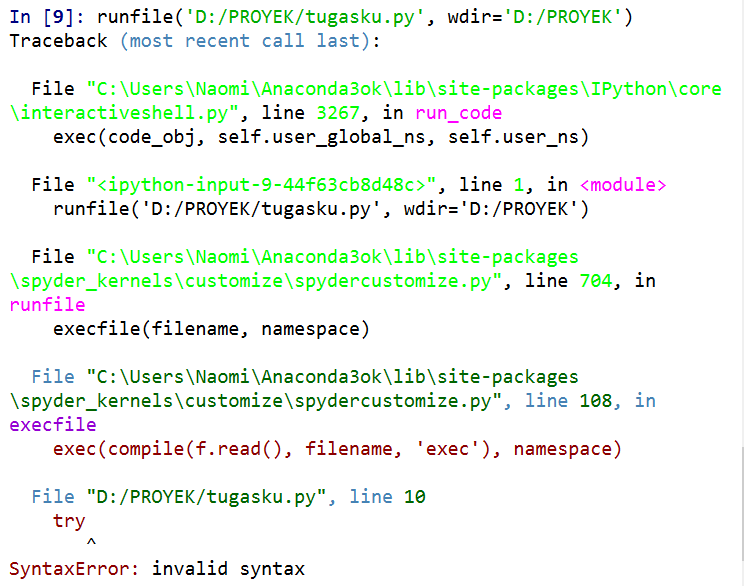
\includegraphics[width=10cm]{gambar2/try1.png}
    \caption{Hasil Contoh Try Except}
    \end{figure}
\end{enumerate}

\newpage
\section{Keterampilan Pemrograman}
\begin{enumerate}
    \item Membuat NPM menggunakan tanda (*)\\
    Contoh Codingan:
    \begin{figure}[!htbp]
    \centering
    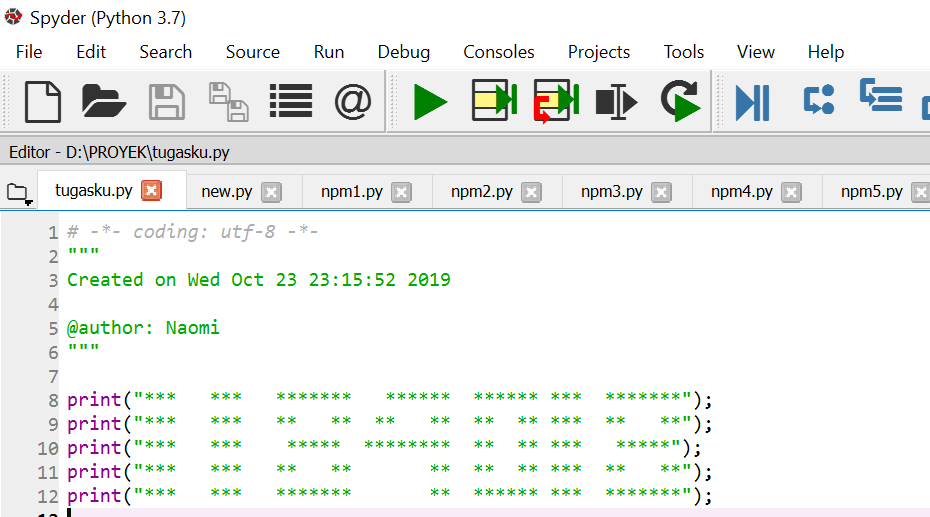
\includegraphics[width=15cm]{gambar2/npm.png}
    \caption{Contoh NPM}
    \end{figure}\\
    Hasil:
    \begin{figure}[!htbp]
    \centering
    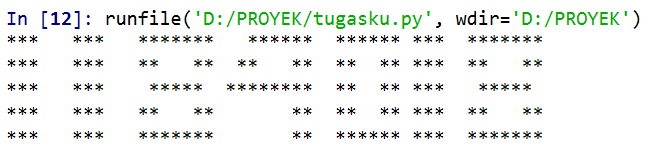
\includegraphics[width=15cm]{gambar2/npm1.png}
    \caption{Hasil Contoh NPM}
    \end{figure}
    
    \newpage
    \item Membuat Program Hello Word dengan input NPM\\ 
    Contoh Codingan:
    \begin{figure}[!htbp]
    \centering
    \includegraphics[width=11cm]{gambar2/halo.png}
    \caption{Contoh Hello Word dengan input NPM}
    \end{figure}
    Hasil:
    \begin{figure}[!htbp]
    \centering
    \includegraphics[width=10cm]{gambar2/halo1.png}
    \caption{Hasil Contoh Hello Word dengan input NPM}
    \end{figure}
    
    \newpage
    \item Program Hello Word menggunakan Input dan Ouput\\
    Contoh Codingan:
    \begin{figure}[!htbp]
    \centering
    \includegraphics[width=12cm]{gambar2/io.png}
    \caption{Contoh Hello Word Input Ouput}
    \end{figure}\\
    Hasil:
    \begin{figure}[!htbp]
    \centering
    \includegraphics[width=13cm]{gambar2/io1.png}
    \caption{Hasil Contoh Hello Input Ouput}
    \end{figure}
    
    \newpage
    \item  Program Hello Word dengan input nama yang disimpan dalam sebuah variabel string bernama NPM dan beri luaran output berupa digit ketiga dari belakang dari variabel NPM.\\
    Contoh Codingan:
    \begin{figure}[!htbp]
    \centering
    \includegraphics[width=13cm]{gambar2/digit.png}
    \caption{Contoh Ouput digit Ketiga}
    \end{figure}\\
    Hasil:
    \begin{figure}[!htbp]
    \centering
    \includegraphics[width=14cm]{gambar2/digit1.png}
    \caption{Hasil Contoh Ouput digit Ketiga}
    \end{figure}
    
    \newpage
    \item Menggunakankan Perulangan dan Kondisi\\
    Contoh Codingan:
    \begin{figure}[!htbp]
    \centering
    \includegraphics[width=13cm]{gambar2/perulangan.png}
    \caption{Contoh menggunakan Perulangan dan Kondisi}
    \end{figure}\\
    Hasil:
    \begin{figure}[!htbp]
    \centering
    \includegraphics[width=14cm]{gambar2/perulangan1.png}
    \caption{Hasil Contoh menggunakan Perulangan dan Kondisi}
    \end{figure}
    
    \newpage
    \item penjumlahan dari seluruh variabel \\
    Contoh Codingan:
    \begin{figure}[!htbp]
    \centering
    \includegraphics[width=13cm]{gambar2/penjumlahan.png}
    \caption{Contoh penjumlahan dari seluruh variabel}
    \end{figure}\\
    Hasil:
    \begin{figure}[!htbp]
    \centering
    \includegraphics[width=14cm]{gambar2/penjumlahan1.png}
    \caption{HasilContoh penjumlahan dari seluruh variabel}
    \end{figure}
    
    \newpage
    \item Bilangan Ganjil \\
    Contoh Codingan:
    \begin{figure}[!htbp]
    \centering
    \includegraphics[width=13cm]{gambar2/ganjil.png}
    \caption{Contoh Bilangan Ganjil}
    \end{figure}\\
    Hasil:
    \begin{figure}[!htbp]
    \centering
    \includegraphics[width=14cm]{gambar2/ganjil1.png}
    \caption{Hasil Contoh Bilangan Ganjil}
    \end{figure}
    
    \newpage
    \item Bilangan Genap \\
    Contoh Codingan:
    \begin{figure}[!htbp]
    \centering
    \includegraphics[width=13cm]{gambar2/genap.png}
    \caption{Contoh Bilangan Genap}
    \end{figure}\\
    Hasil:
    \begin{figure}[!htbp]
    \centering
    \includegraphics[width=14cm]{gambar2/genap1.png}
    \caption{Hasil Contoh Bilangan Genap}
    \end{figure}
    
    \newpage
    \item Bilangan Genap \\
    Contoh Codingan:
    \begin{figure}[!htbp]
    \centering
    \includegraphics[width=13cm]{gambar2/genap.png}
    \caption{Contoh Bilangan Genap}
    \end{figure}\\
    Hasil:
    \begin{figure}[!htbp]
    \centering
    \includegraphics[width=14cm]{gambar2/genap1.png}
    \caption{Hasil Contoh Bilangan Genap}
    \end{figure}
    
    \newpage
    \item Bilangan Prima \\
    Contoh Codingan:
    \begin{figure}[!htbp]
    \centering
    \includegraphics[width=13cm]{gambar2/prim.png}
    \caption{Contoh Bilangan Prima}
    \end{figure}
\end{enumerate}




